\documentclass[twoside]{book}

% Packages required by doxygen
\usepackage{fixltx2e}
\usepackage{calc}
\usepackage{doxygen}
\usepackage[export]{adjustbox} % also loads graphicx
\usepackage{graphicx}
\usepackage[utf8]{inputenc}
\usepackage{makeidx}
\usepackage{multicol}
\usepackage{multirow}
\PassOptionsToPackage{warn}{textcomp}
\usepackage{textcomp}
\usepackage[nointegrals]{wasysym}
\usepackage[table]{xcolor}

% Font selection
\usepackage[T1]{fontenc}
\usepackage[scaled=.90]{helvet}
\usepackage{courier}
\usepackage{amssymb}
\usepackage{sectsty}
\renewcommand{\familydefault}{\sfdefault}
\allsectionsfont{%
  \fontseries{bc}\selectfont%
  \color{darkgray}%
}
\renewcommand{\DoxyLabelFont}{%
  \fontseries{bc}\selectfont%
  \color{darkgray}%
}
\newcommand{\+}{\discretionary{\mbox{\scriptsize$\hookleftarrow$}}{}{}}

% Page & text layout
\usepackage{geometry}
\geometry{%
  a4paper,%
  top=2.5cm,%
  bottom=2.5cm,%
  left=2.5cm,%
  right=2.5cm%
}
\tolerance=750
\hfuzz=15pt
\hbadness=750
\setlength{\emergencystretch}{15pt}
\setlength{\parindent}{0cm}
\setlength{\parskip}{3ex plus 2ex minus 2ex}
\makeatletter
\renewcommand{\paragraph}{%
  \@startsection{paragraph}{4}{0ex}{-1.0ex}{1.0ex}{%
    \normalfont\normalsize\bfseries\SS@parafont%
  }%
}
\renewcommand{\subparagraph}{%
  \@startsection{subparagraph}{5}{0ex}{-1.0ex}{1.0ex}{%
    \normalfont\normalsize\bfseries\SS@subparafont%
  }%
}
\makeatother

% Headers & footers
\usepackage{fancyhdr}
\pagestyle{fancyplain}
\fancyhead[LE]{\fancyplain{}{\bfseries\thepage}}
\fancyhead[CE]{\fancyplain{}{}}
\fancyhead[RE]{\fancyplain{}{\bfseries\leftmark}}
\fancyhead[LO]{\fancyplain{}{\bfseries\rightmark}}
\fancyhead[CO]{\fancyplain{}{}}
\fancyhead[RO]{\fancyplain{}{\bfseries\thepage}}
\fancyfoot[LE]{\fancyplain{}{}}
\fancyfoot[CE]{\fancyplain{}{}}
\fancyfoot[RE]{\fancyplain{}{\bfseries\scriptsize Generated by Doxygen }}
\fancyfoot[LO]{\fancyplain{}{\bfseries\scriptsize Generated by Doxygen }}
\fancyfoot[CO]{\fancyplain{}{}}
\fancyfoot[RO]{\fancyplain{}{}}
\renewcommand{\footrulewidth}{0.4pt}
\renewcommand{\chaptermark}[1]{%
  \markboth{#1}{}%
}
\renewcommand{\sectionmark}[1]{%
  \markright{\thesection\ #1}%
}

% Indices & bibliography
\usepackage{natbib}
\usepackage[titles]{tocloft}
\setcounter{tocdepth}{3}
\setcounter{secnumdepth}{5}
\makeindex

% Hyperlinks (required, but should be loaded last)
\usepackage{ifpdf}
\ifpdf
  \usepackage[pdftex,pagebackref=true]{hyperref}
\else
  \usepackage[ps2pdf,pagebackref=true]{hyperref}
\fi
\hypersetup{%
  colorlinks=true,%
  linkcolor=blue,%
  citecolor=blue,%
  unicode%
}

% Custom commands
\newcommand{\clearemptydoublepage}{%
  \newpage{\pagestyle{empty}\cleardoublepage}%
}

\usepackage{caption}
\captionsetup{labelsep=space,justification=centering,font={bf},singlelinecheck=off,skip=4pt,position=top}

%===== C O N T E N T S =====

\begin{document}

% Titlepage & ToC
\hypersetup{pageanchor=false,
             bookmarksnumbered=true,
             pdfencoding=unicode
            }
\pagenumbering{alph}
\begin{titlepage}
\vspace*{7cm}
\begin{center}%
{\Large Little\+War\+Game }\\
\vspace*{1cm}
{\large Generated by Doxygen 1.8.14}\\
\end{center}
\end{titlepage}
\clearemptydoublepage
\pagenumbering{roman}
\tableofcontents
\clearemptydoublepage
\pagenumbering{arabic}
\hypersetup{pageanchor=true}

%--- Begin generated contents ---
\chapter{Little\+War\+Game}
\label{md_README}
\Hypertarget{md_README}
This is just a Little War Game without any ambition or even graphism.

\subsection*{What do you need}

Even if this is really simple to find what you need to run properly this project, this is a list of needed software \+:


\begin{DoxyEnumerate}
\item Apache or Nginx server (or other maybe, I don\textquotesingle{}t really care)
\item Mysql or Maria\+DB
\item Doxygen
\item Graphivz (for Doxygen graphs)
\item Mysql\+Work\+Bench (to read the M\+PD if you want to see it) 
\end{DoxyEnumerate}
\chapter{Class Index}
\section{Class List}
Here are the classes, structs, unions and interfaces with brief descriptions\+:\begin{DoxyCompactList}
\item\contentsline{section}{\mbox{\hyperlink{classInventory}{Inventory}} \\*This class store all Ressources belonging to another object like a \mbox{\hyperlink{classTemple}{Temple}} or a \mbox{\hyperlink{classVillage}{Village}} }{\pageref{classInventory}}{}
\item\contentsline{section}{\mbox{\hyperlink{classMember}{Member}} \\*This class is the core of the projet because it store all informations about villages, so all informations about the member }{\pageref{classMember}}{}
\item\contentsline{section}{\mbox{\hyperlink{classSQL}{S\+QL}} }{\pageref{classSQL}}{}
\item\contentsline{section}{\mbox{\hyperlink{classTemple}{Temple}} }{\pageref{classTemple}}{}
\item\contentsline{section}{\mbox{\hyperlink{classVillage}{Village}} \\*This class is the core of the game because all other objects are link to it }{\pageref{classVillage}}{}
\end{DoxyCompactList}

\chapter{File Index}
\section{File List}
Here is a list of all documented files with brief descriptions\+:\begin{DoxyCompactList}
\item\contentsline{section}{Controleurs/\mbox{\hyperlink{Controleurs_2accueil_8php}{accueil.\+php}} \\*This script manage two case \+: }{\pageref{Controleurs_2accueil_8php}}{}
\item\contentsline{section}{Controleurs/\mbox{\hyperlink{connexion_8php}{connexion.\+php}} \\*This script job is te find if the member exist and store all data about it in S\+E\+S\+S\+I\+ON to limit the amount of needed \mbox{\hyperlink{classSQL}{S\+QL}} request on each page (0 until the member ask for some modifications) }{\pageref{connexion_8php}}{}
\end{DoxyCompactList}

\chapter{Class Documentation}
\hypertarget{classInventory}{}\section{Inventory Class Reference}
\label{classInventory}\index{Inventory@{Inventory}}


This class store all Ressources belonging to another object like a \mbox{\hyperlink{classTemple}{Temple}} or a \mbox{\hyperlink{classVillage}{Village}}.  




Collaboration diagram for Inventory\+:
\nopagebreak
\begin{figure}[H]
\begin{center}
\leavevmode
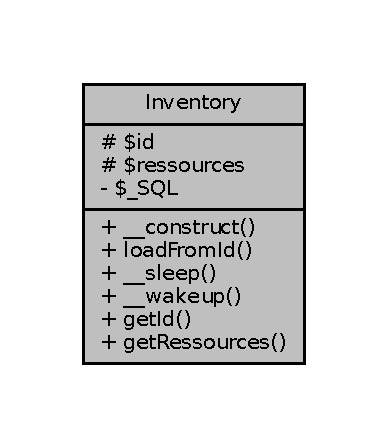
\includegraphics[width=186pt]{classInventory__coll__graph}
\end{center}
\end{figure}
\subsection*{Public Member Functions}
\begin{DoxyCompactItemize}
\item 
\mbox{\hyperlink{classInventory_ad590054ec1e295007c7a7f14ecd12ac5}{\+\_\+\+\_\+construct}} (\$id)
\begin{DoxyCompactList}\small\item\em Constructor for the class \mbox{\hyperlink{classInventory}{Inventory}}. \end{DoxyCompactList}\item 
\mbox{\hyperlink{classInventory_ad5fa182aefcd1e26ae373b70bd23a7a5}{load\+From\+Id}} ()
\begin{DoxyCompactList}\small\item\em This method load the ressources of this inventory based on the id attribute. \end{DoxyCompactList}\item 
\mbox{\hyperlink{classInventory_af7c8af72b921f5d7ba545d62378b113b}{\+\_\+\+\_\+sleep}} ()
\begin{DoxyCompactList}\small\item\em This method define the fields to save when we ask P\+HP for serialize a \mbox{\hyperlink{classInventory}{Inventory}} object. \end{DoxyCompactList}\item 
\mbox{\Hypertarget{classInventory_ada9aa6a6e88be3d5fce6b318e459664d}\label{classInventory_ada9aa6a6e88be3d5fce6b318e459664d}} 
\mbox{\hyperlink{classInventory_ada9aa6a6e88be3d5fce6b318e459664d}{\+\_\+\+\_\+wakeup}} ()
\begin{DoxyCompactList}\small\item\em This method get an reference on the current \mbox{\hyperlink{classSQL}{S\+QL}} instance when P\+HP deserialize a \mbox{\hyperlink{classInventory}{Inventory}} object. \end{DoxyCompactList}\item 
\mbox{\hyperlink{classInventory_ae571fc67c0f3bb9582de755f624ba680}{get\+Id}} ()
\begin{DoxyCompactList}\small\item\em Getter for \mbox{\hyperlink{classInventory}{Inventory}} ID. \end{DoxyCompactList}\item 
\mbox{\hyperlink{classInventory_a9b570bb7650509c786bc066347229979}{get\+Ressources}} ()
\begin{DoxyCompactList}\small\item\em Getter for \mbox{\hyperlink{classInventory}{Inventory}} Ressources list. \end{DoxyCompactList}\end{DoxyCompactItemize}
\subsection*{Protected Attributes}
\begin{DoxyCompactItemize}
\item 
\mbox{\Hypertarget{classInventory_a938439393bff41626879c81b27fa3eb1}\label{classInventory_a938439393bff41626879c81b27fa3eb1}} 
\mbox{\hyperlink{classInventory_a938439393bff41626879c81b27fa3eb1}{\$id}}
\begin{DoxyCompactList}\small\item\em The \mbox{\hyperlink{classInventory}{Inventory}} ID. \end{DoxyCompactList}\item 
\mbox{\Hypertarget{classInventory_ae2de638a5d5b2175cea1327dd6a1097d}\label{classInventory_ae2de638a5d5b2175cea1327dd6a1097d}} 
\mbox{\hyperlink{classInventory_ae2de638a5d5b2175cea1327dd6a1097d}{\$ressources}} = array()
\begin{DoxyCompactList}\small\item\em The Ressources list in this inventory. \end{DoxyCompactList}\end{DoxyCompactItemize}
\subsection*{Private Attributes}
\begin{DoxyCompactItemize}
\item 
\mbox{\Hypertarget{classInventory_a7097eb9666f0d9e70ef7d0b1ef770cb5}\label{classInventory_a7097eb9666f0d9e70ef7d0b1ef770cb5}} 
\mbox{\hyperlink{classInventory_a7097eb9666f0d9e70ef7d0b1ef770cb5}{\$\+\_\+\+S\+QL}}
\begin{DoxyCompactList}\small\item\em Reference on the \mbox{\hyperlink{classSQL}{S\+QL}} connexion. \end{DoxyCompactList}\end{DoxyCompactItemize}


\subsection{Detailed Description}
This class store all Ressources belonging to another object like a \mbox{\hyperlink{classTemple}{Temple}} or a \mbox{\hyperlink{classVillage}{Village}}. 

\subsection{Constructor \& Destructor Documentation}
\mbox{\Hypertarget{classInventory_ad590054ec1e295007c7a7f14ecd12ac5}\label{classInventory_ad590054ec1e295007c7a7f14ecd12ac5}} 
\index{Inventory@{Inventory}!\+\_\+\+\_\+construct@{\+\_\+\+\_\+construct}}
\index{\+\_\+\+\_\+construct@{\+\_\+\+\_\+construct}!Inventory@{Inventory}}
\subsubsection{\texorpdfstring{\+\_\+\+\_\+construct()}{\_\_construct()}}
{\footnotesize\ttfamily Inventory\+::\+\_\+\+\_\+construct (\begin{DoxyParamCaption}\item[{}]{\$id }\end{DoxyParamCaption})}



Constructor for the class \mbox{\hyperlink{classInventory}{Inventory}}. 


\begin{DoxyParams}{Parameters}
{\em \$id} & the \mbox{\hyperlink{classInventory}{Inventory}} ID \\
\hline
\end{DoxyParams}
\begin{DoxyReturn}{Returns}
returns the initialized \mbox{\hyperlink{classInventory}{Inventory}} object 
\end{DoxyReturn}


\subsection{Member Function Documentation}
\mbox{\Hypertarget{classInventory_af7c8af72b921f5d7ba545d62378b113b}\label{classInventory_af7c8af72b921f5d7ba545d62378b113b}} 
\index{Inventory@{Inventory}!\+\_\+\+\_\+sleep@{\+\_\+\+\_\+sleep}}
\index{\+\_\+\+\_\+sleep@{\+\_\+\+\_\+sleep}!Inventory@{Inventory}}
\subsubsection{\texorpdfstring{\+\_\+\+\_\+sleep()}{\_\_sleep()}}
{\footnotesize\ttfamily Inventory\+::\+\_\+\+\_\+sleep (\begin{DoxyParamCaption}{ }\end{DoxyParamCaption})}



This method define the fields to save when we ask P\+HP for serialize a \mbox{\hyperlink{classInventory}{Inventory}} object. 

\begin{DoxyReturn}{Returns}
returns the list of attribute to save 
\end{DoxyReturn}
\mbox{\Hypertarget{classInventory_ae571fc67c0f3bb9582de755f624ba680}\label{classInventory_ae571fc67c0f3bb9582de755f624ba680}} 
\index{Inventory@{Inventory}!get\+Id@{get\+Id}}
\index{get\+Id@{get\+Id}!Inventory@{Inventory}}
\subsubsection{\texorpdfstring{get\+Id()}{getId()}}
{\footnotesize\ttfamily Inventory\+::get\+Id (\begin{DoxyParamCaption}{ }\end{DoxyParamCaption})}



Getter for \mbox{\hyperlink{classInventory}{Inventory}} ID. 

\begin{DoxyReturn}{Returns}
returns the \mbox{\hyperlink{classInventory}{Inventory}} ID 
\end{DoxyReturn}
\mbox{\Hypertarget{classInventory_a9b570bb7650509c786bc066347229979}\label{classInventory_a9b570bb7650509c786bc066347229979}} 
\index{Inventory@{Inventory}!get\+Ressources@{get\+Ressources}}
\index{get\+Ressources@{get\+Ressources}!Inventory@{Inventory}}
\subsubsection{\texorpdfstring{get\+Ressources()}{getRessources()}}
{\footnotesize\ttfamily Inventory\+::get\+Ressources (\begin{DoxyParamCaption}{ }\end{DoxyParamCaption})}



Getter for \mbox{\hyperlink{classInventory}{Inventory}} Ressources list. 

\begin{DoxyReturn}{Returns}
returns the \mbox{\hyperlink{classInventory}{Inventory}} Ressources list 
\end{DoxyReturn}
\mbox{\Hypertarget{classInventory_ad5fa182aefcd1e26ae373b70bd23a7a5}\label{classInventory_ad5fa182aefcd1e26ae373b70bd23a7a5}} 
\index{Inventory@{Inventory}!load\+From\+Id@{load\+From\+Id}}
\index{load\+From\+Id@{load\+From\+Id}!Inventory@{Inventory}}
\subsubsection{\texorpdfstring{load\+From\+Id()}{loadFromId()}}
{\footnotesize\ttfamily Inventory\+::load\+From\+Id (\begin{DoxyParamCaption}{ }\end{DoxyParamCaption})}



This method load the ressources of this inventory based on the id attribute. 

\begin{DoxyReturn}{Returns}
returns true if it\textquotesingle{}s succeed 
\end{DoxyReturn}


The documentation for this class was generated from the following file\+:\begin{DoxyCompactItemize}
\item 
Classes/Inventory.\+php\end{DoxyCompactItemize}

\hypertarget{classMember}{}\section{Member Class Reference}
\label{classMember}\index{Member@{Member}}


This class is the core of the projet because it store all informations about villages, so all informations about the member.  




Collaboration diagram for Member\+:\nopagebreak
\begin{figure}[H]
\begin{center}
\leavevmode
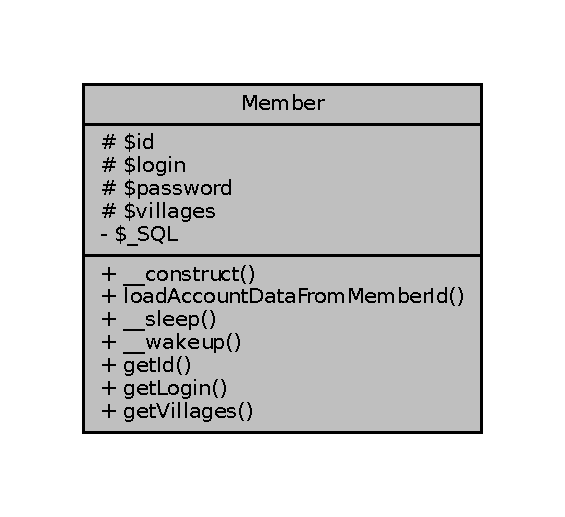
\includegraphics[width=271pt]{classMember__coll__graph}
\end{center}
\end{figure}
\subsection*{Public Member Functions}
\begin{DoxyCompactItemize}
\item 
\mbox{\hyperlink{classMember_adfd583576ca6cc09f0f8868ac7c75f3a}{\+\_\+\+\_\+construct}} (\$id)
\begin{DoxyCompactList}\small\item\em Constructor for the class \mbox{\hyperlink{classMember}{Member}}. \end{DoxyCompactList}\item 
\mbox{\hyperlink{classMember_a9624c3631bc10fbc592380353e537928}{load\+Account\+Data\+From\+Member\+Id}} ()
\begin{DoxyCompactList}\small\item\em This method load all data about this \mbox{\hyperlink{classMember}{Member}} to store them in S\+E\+S\+S\+I\+ON. \end{DoxyCompactList}\item 
\mbox{\hyperlink{classMember_a08bdbef60afdd66ea4e1f3c2404d6b6f}{\+\_\+\+\_\+sleep}} ()
\begin{DoxyCompactList}\small\item\em This method define the fields to save when we ask P\+HP for serialize a \mbox{\hyperlink{classMember}{Member}} object. \end{DoxyCompactList}\item 
\mbox{\Hypertarget{classMember_ad9f31b2c9942ffcf8f6cd99590307e66}\label{classMember_ad9f31b2c9942ffcf8f6cd99590307e66}} 
\mbox{\hyperlink{classMember_ad9f31b2c9942ffcf8f6cd99590307e66}{\+\_\+\+\_\+wakeup}} ()
\begin{DoxyCompactList}\small\item\em This method get an reference on the current \mbox{\hyperlink{classSQL}{S\+QL}} instance when P\+HP deserialize a \mbox{\hyperlink{classMember}{Member}} object. \end{DoxyCompactList}\item 
\mbox{\hyperlink{classMember_a4c2dcf5c05164f9575bc01237756109f}{get\+Id}} ()
\begin{DoxyCompactList}\small\item\em Getter for \mbox{\hyperlink{classMember}{Member}} ID. \end{DoxyCompactList}\item 
\mbox{\hyperlink{classMember_a24f3ec8686336825d65d4c3ce1ca995a}{get\+Login}} ()
\begin{DoxyCompactList}\small\item\em Getter for \mbox{\hyperlink{classMember}{Member}} Login. \end{DoxyCompactList}\item 
\mbox{\hyperlink{classMember_a8fffb15679150731080b062cf4770f7d}{get\+Villages}} ()
\begin{DoxyCompactList}\small\item\em Getter for \mbox{\hyperlink{classMember}{Member}} \mbox{\hyperlink{classVillage}{Village}} list. \end{DoxyCompactList}\end{DoxyCompactItemize}
\subsection*{Protected Attributes}
\begin{DoxyCompactItemize}
\item 
\mbox{\Hypertarget{classMember_aa65bcf3ccbc37e49a1c58b6ce3b7a386}\label{classMember_aa65bcf3ccbc37e49a1c58b6ce3b7a386}} 
\mbox{\hyperlink{classMember_aa65bcf3ccbc37e49a1c58b6ce3b7a386}{\$id}}
\begin{DoxyCompactList}\small\item\em The \mbox{\hyperlink{classMember}{Member}} ID. \end{DoxyCompactList}\item 
\mbox{\Hypertarget{classMember_a07c5e5efcaa4a129a3228424a0d58f57}\label{classMember_a07c5e5efcaa4a129a3228424a0d58f57}} 
\mbox{\hyperlink{classMember_a07c5e5efcaa4a129a3228424a0d58f57}{\$login}}
\begin{DoxyCompactList}\small\item\em The \mbox{\hyperlink{classMember}{Member}} login. \end{DoxyCompactList}\item 
\mbox{\Hypertarget{classMember_a8ed491893ed68a3471ee7bbcfc746080}\label{classMember_a8ed491893ed68a3471ee7bbcfc746080}} 
\mbox{\hyperlink{classMember_a8ed491893ed68a3471ee7bbcfc746080}{\$password}}
\begin{DoxyCompactList}\small\item\em The \mbox{\hyperlink{classMember}{Member}} password (hash) \end{DoxyCompactList}\item 
\mbox{\Hypertarget{classMember_aa875e5b954df4f039d060ed033286efb}\label{classMember_aa875e5b954df4f039d060ed033286efb}} 
\mbox{\hyperlink{classMember_aa875e5b954df4f039d060ed033286efb}{\$villages}}
\begin{DoxyCompactList}\small\item\em List of \mbox{\hyperlink{classVillage}{Village}} object. \end{DoxyCompactList}\end{DoxyCompactItemize}
\subsection*{Private Attributes}
\begin{DoxyCompactItemize}
\item 
\mbox{\Hypertarget{classMember_ab4eb199b244a08e19c2804469e249b2b}\label{classMember_ab4eb199b244a08e19c2804469e249b2b}} 
\mbox{\hyperlink{classMember_ab4eb199b244a08e19c2804469e249b2b}{\$\+\_\+\+S\+QL}}
\begin{DoxyCompactList}\small\item\em Reference on the \mbox{\hyperlink{classSQL}{S\+QL}} connexion. \end{DoxyCompactList}\end{DoxyCompactItemize}


\subsection{Detailed Description}
This class is the core of the projet because it store all informations about villages, so all informations about the member. 

\subsection{Constructor \& Destructor Documentation}
\mbox{\Hypertarget{classMember_adfd583576ca6cc09f0f8868ac7c75f3a}\label{classMember_adfd583576ca6cc09f0f8868ac7c75f3a}} 
\index{Member@{Member}!\+\_\+\+\_\+construct@{\+\_\+\+\_\+construct}}
\index{\+\_\+\+\_\+construct@{\+\_\+\+\_\+construct}!Member@{Member}}
\subsubsection{\texorpdfstring{\+\_\+\+\_\+construct()}{\_\_construct()}}
{\footnotesize\ttfamily Member\+::\+\_\+\+\_\+construct (\begin{DoxyParamCaption}\item[{}]{\$id }\end{DoxyParamCaption})}



Constructor for the class \mbox{\hyperlink{classMember}{Member}}. 


\begin{DoxyParams}{Parameters}
{\em \$id} & the \mbox{\hyperlink{classMember}{Member}} ID \\
\hline
\end{DoxyParams}
\begin{DoxyReturn}{Returns}
returns the initialized \mbox{\hyperlink{classMember}{Member}} object 
\end{DoxyReturn}


\subsection{Member Function Documentation}
\mbox{\Hypertarget{classMember_a08bdbef60afdd66ea4e1f3c2404d6b6f}\label{classMember_a08bdbef60afdd66ea4e1f3c2404d6b6f}} 
\index{Member@{Member}!\+\_\+\+\_\+sleep@{\+\_\+\+\_\+sleep}}
\index{\+\_\+\+\_\+sleep@{\+\_\+\+\_\+sleep}!Member@{Member}}
\subsubsection{\texorpdfstring{\+\_\+\+\_\+sleep()}{\_\_sleep()}}
{\footnotesize\ttfamily Member\+::\+\_\+\+\_\+sleep (\begin{DoxyParamCaption}{ }\end{DoxyParamCaption})}



This method define the fields to save when we ask P\+HP for serialize a \mbox{\hyperlink{classMember}{Member}} object. 

\begin{DoxyReturn}{Returns}
returns the list of attribute to save 
\end{DoxyReturn}
\mbox{\Hypertarget{classMember_a4c2dcf5c05164f9575bc01237756109f}\label{classMember_a4c2dcf5c05164f9575bc01237756109f}} 
\index{Member@{Member}!get\+Id@{get\+Id}}
\index{get\+Id@{get\+Id}!Member@{Member}}
\subsubsection{\texorpdfstring{get\+Id()}{getId()}}
{\footnotesize\ttfamily Member\+::get\+Id (\begin{DoxyParamCaption}{ }\end{DoxyParamCaption})}



Getter for \mbox{\hyperlink{classMember}{Member}} ID. 

\begin{DoxyReturn}{Returns}
returns the \mbox{\hyperlink{classMember}{Member}} ID 
\end{DoxyReturn}
\mbox{\Hypertarget{classMember_a24f3ec8686336825d65d4c3ce1ca995a}\label{classMember_a24f3ec8686336825d65d4c3ce1ca995a}} 
\index{Member@{Member}!get\+Login@{get\+Login}}
\index{get\+Login@{get\+Login}!Member@{Member}}
\subsubsection{\texorpdfstring{get\+Login()}{getLogin()}}
{\footnotesize\ttfamily Member\+::get\+Login (\begin{DoxyParamCaption}{ }\end{DoxyParamCaption})}



Getter for \mbox{\hyperlink{classMember}{Member}} Login. 

\begin{DoxyReturn}{Returns}
returns the \mbox{\hyperlink{classMember}{Member}} Login 
\end{DoxyReturn}
\mbox{\Hypertarget{classMember_a8fffb15679150731080b062cf4770f7d}\label{classMember_a8fffb15679150731080b062cf4770f7d}} 
\index{Member@{Member}!get\+Villages@{get\+Villages}}
\index{get\+Villages@{get\+Villages}!Member@{Member}}
\subsubsection{\texorpdfstring{get\+Villages()}{getVillages()}}
{\footnotesize\ttfamily Member\+::get\+Villages (\begin{DoxyParamCaption}{ }\end{DoxyParamCaption})}



Getter for \mbox{\hyperlink{classMember}{Member}} \mbox{\hyperlink{classVillage}{Village}} list. 

\begin{DoxyReturn}{Returns}
returns the \mbox{\hyperlink{classMember}{Member}} \mbox{\hyperlink{classVillage}{Village}} list 
\end{DoxyReturn}
\mbox{\Hypertarget{classMember_a9624c3631bc10fbc592380353e537928}\label{classMember_a9624c3631bc10fbc592380353e537928}} 
\index{Member@{Member}!load\+Account\+Data\+From\+Member\+Id@{load\+Account\+Data\+From\+Member\+Id}}
\index{load\+Account\+Data\+From\+Member\+Id@{load\+Account\+Data\+From\+Member\+Id}!Member@{Member}}
\subsubsection{\texorpdfstring{load\+Account\+Data\+From\+Member\+Id()}{loadAccountDataFromMemberId()}}
{\footnotesize\ttfamily Member\+::load\+Account\+Data\+From\+Member\+Id (\begin{DoxyParamCaption}{ }\end{DoxyParamCaption})}



This method load all data about this \mbox{\hyperlink{classMember}{Member}} to store them in S\+E\+S\+S\+I\+ON. 


\begin{DoxyItemize}
\item \mbox{\hyperlink{classVillage}{Village}} list
\begin{DoxyItemize}
\item Workers in the \mbox{\hyperlink{classVillage}{Village}}
\item \mbox{\hyperlink{classTemple}{Temple}} in the \mbox{\hyperlink{classVillage}{Village}}
\item Buildings in the \mbox{\hyperlink{classVillage}{Village}} \begin{DoxyReturn}{Returns}
returns true if it\textquotesingle{}s succeed, false in the other case 
\end{DoxyReturn}

\end{DoxyItemize}
\end{DoxyItemize}Here is the call graph for this function\+:
\nopagebreak
\begin{figure}[H]
\begin{center}
\leavevmode
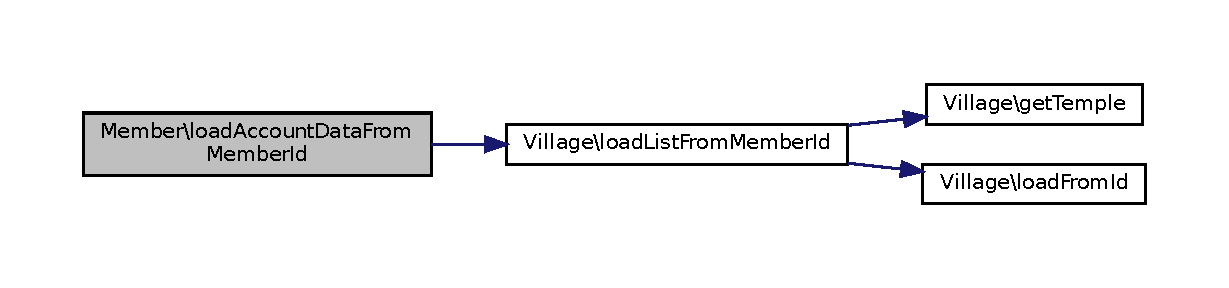
\includegraphics[width=350pt]{classMember_a9624c3631bc10fbc592380353e537928_cgraph}
\end{center}
\end{figure}


The documentation for this class was generated from the following file\+:\begin{DoxyCompactItemize}
\item 
Classes/Member.\+php\end{DoxyCompactItemize}

\hypertarget{classSQL}{}\section{S\+QL Class Reference}
\label{classSQL}\index{S\+QL@{S\+QL}}


Collaboration diagram for S\+QL\+:\nopagebreak
\begin{figure}[H]
\begin{center}
\leavevmode
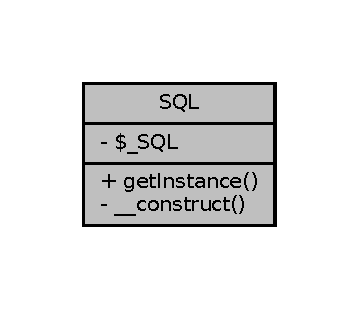
\includegraphics[width=172pt]{classSQL__coll__graph}
\end{center}
\end{figure}
\subsection*{Static Public Member Functions}
\begin{DoxyCompactItemize}
\item 
\mbox{\Hypertarget{classSQL_a7704a7213939ea2120ca2abee226d08e}\label{classSQL_a7704a7213939ea2120ca2abee226d08e}} 
static {\bfseries get\+Instance} ()
\end{DoxyCompactItemize}
\subsection*{Static Private Attributes}
\begin{DoxyCompactItemize}
\item 
\mbox{\Hypertarget{classSQL_aa96548c10c0df9772168e13dd60ec4cf}\label{classSQL_aa96548c10c0df9772168e13dd60ec4cf}} 
static {\bfseries \$\+\_\+\+S\+QL} = null
\end{DoxyCompactItemize}


The documentation for this class was generated from the following file\+:\begin{DoxyCompactItemize}
\item 
Classes/S\+Q\+L.\+php\end{DoxyCompactItemize}

\hypertarget{classTemple}{}\section{Temple Class Reference}
\label{classTemple}\index{Temple@{Temple}}


Collaboration diagram for Temple\+:
\nopagebreak
\begin{figure}[H]
\begin{center}
\leavevmode
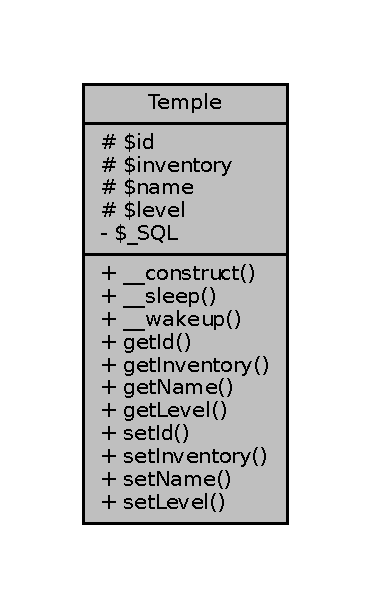
\includegraphics[width=178pt]{classTemple__coll__graph}
\end{center}
\end{figure}
\subsection*{Public Member Functions}
\begin{DoxyCompactItemize}
\item 
\mbox{\Hypertarget{classTemple_a4ab81135c56914a761d573a979d3d02b}\label{classTemple_a4ab81135c56914a761d573a979d3d02b}} 
{\bfseries \+\_\+\+\_\+construct} (\$id)
\item 
\mbox{\hyperlink{classTemple_a08700fe7671bb090ddb042a65a452609}{\+\_\+\+\_\+sleep}} ()
\begin{DoxyCompactList}\small\item\em This method define the fields to save when we ask P\+HP for serialize a \mbox{\hyperlink{classTemple}{Temple}} object. \end{DoxyCompactList}\item 
\mbox{\Hypertarget{classTemple_a7412906ca0259c9c93fa8fd39f776a2a}\label{classTemple_a7412906ca0259c9c93fa8fd39f776a2a}} 
\mbox{\hyperlink{classTemple_a7412906ca0259c9c93fa8fd39f776a2a}{\+\_\+\+\_\+wakeup}} ()
\begin{DoxyCompactList}\small\item\em This method get an reference on the current \mbox{\hyperlink{classSQL}{S\+QL}} instance when P\+HP deserialize a \mbox{\hyperlink{classTemple}{Temple}} object. \end{DoxyCompactList}\item 
\mbox{\Hypertarget{classTemple_ae6cd1081e13a58adb55d7f2825ad1768}\label{classTemple_ae6cd1081e13a58adb55d7f2825ad1768}} 
{\bfseries get\+Id} ()
\item 
\mbox{\Hypertarget{classTemple_a91b5b70bc92fe67da3f5f248411fa4a3}\label{classTemple_a91b5b70bc92fe67da3f5f248411fa4a3}} 
{\bfseries get\+Inventory} ()
\item 
\mbox{\Hypertarget{classTemple_a5f8a7e744c00d4e04e099dff3fd5db83}\label{classTemple_a5f8a7e744c00d4e04e099dff3fd5db83}} 
{\bfseries get\+Name} ()
\item 
\mbox{\Hypertarget{classTemple_a7f7c7d1add89ba9ad3900e8690d8f3a7}\label{classTemple_a7f7c7d1add89ba9ad3900e8690d8f3a7}} 
{\bfseries get\+Level} ()
\item 
\mbox{\Hypertarget{classTemple_a7a97675febdc1f8802437fdb40b1e0fd}\label{classTemple_a7a97675febdc1f8802437fdb40b1e0fd}} 
{\bfseries set\+Id} (\$id)
\item 
\mbox{\Hypertarget{classTemple_aefa4371cdcd6f1bcbe7a342823c0cd79}\label{classTemple_aefa4371cdcd6f1bcbe7a342823c0cd79}} 
{\bfseries set\+Inventory} (\$inventory)
\item 
\mbox{\Hypertarget{classTemple_a381f5fb042fe423b7a920c32fa0655f4}\label{classTemple_a381f5fb042fe423b7a920c32fa0655f4}} 
{\bfseries set\+Name} (\$name)
\item 
\mbox{\Hypertarget{classTemple_a11af9c5c45b7b3155bac6d48eb950e0c}\label{classTemple_a11af9c5c45b7b3155bac6d48eb950e0c}} 
{\bfseries set\+Level} (\$level)
\end{DoxyCompactItemize}
\subsection*{Protected Attributes}
\begin{DoxyCompactItemize}
\item 
\mbox{\Hypertarget{classTemple_a47f629bab7bfc62cfad416e1483d9909}\label{classTemple_a47f629bab7bfc62cfad416e1483d9909}} 
{\bfseries \$id}
\item 
\mbox{\Hypertarget{classTemple_a24b4a0670b93e74d9dd94a40f8d5d356}\label{classTemple_a24b4a0670b93e74d9dd94a40f8d5d356}} 
{\bfseries \$inventory}
\item 
\mbox{\Hypertarget{classTemple_af8843aab4c64cf78abb4183d723297cd}\label{classTemple_af8843aab4c64cf78abb4183d723297cd}} 
{\bfseries \$name}
\item 
\mbox{\Hypertarget{classTemple_a7a8c0084e0207f83b694d52b5ebea08c}\label{classTemple_a7a8c0084e0207f83b694d52b5ebea08c}} 
{\bfseries \$level}
\end{DoxyCompactItemize}
\subsection*{Private Attributes}
\begin{DoxyCompactItemize}
\item 
\mbox{\Hypertarget{classTemple_a04fdd3e820c9a6ea4b01b96474e8e8d7}\label{classTemple_a04fdd3e820c9a6ea4b01b96474e8e8d7}} 
{\bfseries \$\+\_\+\+S\+QL}
\end{DoxyCompactItemize}


\subsection{Member Function Documentation}
\mbox{\Hypertarget{classTemple_a08700fe7671bb090ddb042a65a452609}\label{classTemple_a08700fe7671bb090ddb042a65a452609}} 
\index{Temple@{Temple}!\+\_\+\+\_\+sleep@{\+\_\+\+\_\+sleep}}
\index{\+\_\+\+\_\+sleep@{\+\_\+\+\_\+sleep}!Temple@{Temple}}
\subsubsection{\texorpdfstring{\+\_\+\+\_\+sleep()}{\_\_sleep()}}
{\footnotesize\ttfamily Temple\+::\+\_\+\+\_\+sleep (\begin{DoxyParamCaption}{ }\end{DoxyParamCaption})}



This method define the fields to save when we ask P\+HP for serialize a \mbox{\hyperlink{classTemple}{Temple}} object. 

\begin{DoxyReturn}{Returns}
returns the list of attribute to save 
\end{DoxyReturn}


The documentation for this class was generated from the following file\+:\begin{DoxyCompactItemize}
\item 
Classes/Temple.\+php\end{DoxyCompactItemize}

\hypertarget{classVillage}{}\section{Village Class Reference}
\label{classVillage}\index{Village@{Village}}


This class is the core of the game because all other objects are link to it.  




Collaboration diagram for Village\+:
\nopagebreak
\begin{figure}[H]
\begin{center}
\leavevmode
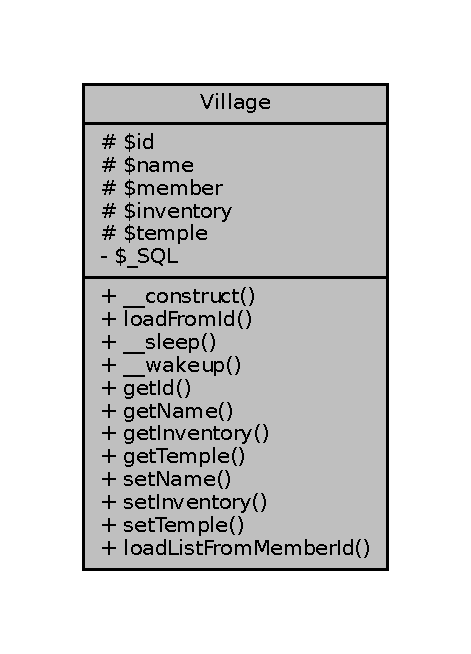
\includegraphics[width=226pt]{classVillage__coll__graph}
\end{center}
\end{figure}
\subsection*{Public Member Functions}
\begin{DoxyCompactItemize}
\item 
\mbox{\hyperlink{classVillage_a2e242983f34bdede6730316edccfa988}{\+\_\+\+\_\+construct}} (\$id)
\begin{DoxyCompactList}\small\item\em Constructor for the class \mbox{\hyperlink{classVillage}{Village}}. \end{DoxyCompactList}\item 
\mbox{\hyperlink{classVillage_a32709e6efc8c58dcedea9727cfa44973}{load\+From\+Id}} ()
\begin{DoxyCompactList}\small\item\em This method load the data about this \mbox{\hyperlink{classVillage}{Village}} \+: \end{DoxyCompactList}\item 
\mbox{\hyperlink{classVillage_a0bea180246dc3d1d6916cf295f57cb7a}{\+\_\+\+\_\+sleep}} ()
\begin{DoxyCompactList}\small\item\em This method define the fields to save when we ask P\+HP for serialize a \mbox{\hyperlink{classVillage}{Village}} object. \end{DoxyCompactList}\item 
\mbox{\Hypertarget{classVillage_a0ab7b982773c3eb1b10a7ed314b87c42}\label{classVillage_a0ab7b982773c3eb1b10a7ed314b87c42}} 
\mbox{\hyperlink{classVillage_a0ab7b982773c3eb1b10a7ed314b87c42}{\+\_\+\+\_\+wakeup}} ()
\begin{DoxyCompactList}\small\item\em This method get an reference on the current \mbox{\hyperlink{classSQL}{S\+QL}} instance when P\+HP deserialize a \mbox{\hyperlink{classVillage}{Village}} object. \end{DoxyCompactList}\item 
\mbox{\hyperlink{classVillage_a5729e2071e18f7cd31bb65b771d51a59}{get\+Id}} ()
\begin{DoxyCompactList}\small\item\em Getter for \mbox{\hyperlink{classVillage}{Village}} ID. \end{DoxyCompactList}\item 
\mbox{\hyperlink{classVillage_a42259e980f432193138a5cad1d48866f}{get\+Name}} ()
\begin{DoxyCompactList}\small\item\em Getter for \mbox{\hyperlink{classVillage}{Village}} name. \end{DoxyCompactList}\item 
\mbox{\hyperlink{classVillage_a9c8354350df0f41853c44799625345d4}{get\+Inventory}} ()
\begin{DoxyCompactList}\small\item\em Getter for \mbox{\hyperlink{classVillage}{Village}} \mbox{\hyperlink{classInventory}{Inventory}}. \end{DoxyCompactList}\item 
\mbox{\hyperlink{classVillage_a75b6534f378f19bb04147fd5c85a1de9}{get\+Temple}} ()
\begin{DoxyCompactList}\small\item\em Getter for \mbox{\hyperlink{classVillage}{Village}} \mbox{\hyperlink{classTemple}{Temple}}. \end{DoxyCompactList}\item 
\mbox{\Hypertarget{classVillage_a3618cf8e4e09b2b76ee0761f954ea2e5}\label{classVillage_a3618cf8e4e09b2b76ee0761f954ea2e5}} 
\mbox{\hyperlink{classVillage_a3618cf8e4e09b2b76ee0761f954ea2e5}{set\+Name}} (\$name)
\begin{DoxyCompactList}\small\item\em Setter for \mbox{\hyperlink{classVillage}{Village}} name. \end{DoxyCompactList}\item 
\mbox{\Hypertarget{classVillage_a03a12402942f6c93091dd6e8bf4c2fee}\label{classVillage_a03a12402942f6c93091dd6e8bf4c2fee}} 
\mbox{\hyperlink{classVillage_a03a12402942f6c93091dd6e8bf4c2fee}{set\+Inventory}} (\$inventory)
\begin{DoxyCompactList}\small\item\em Setter for \mbox{\hyperlink{classVillage}{Village}} \mbox{\hyperlink{classInventory}{Inventory}}. \end{DoxyCompactList}\item 
\mbox{\Hypertarget{classVillage_a5ec3883315293ce70ff632aa088548fd}\label{classVillage_a5ec3883315293ce70ff632aa088548fd}} 
\mbox{\hyperlink{classVillage_a5ec3883315293ce70ff632aa088548fd}{set\+Temple}} (\$temple)
\begin{DoxyCompactList}\small\item\em Setter for \mbox{\hyperlink{classVillage}{Village}} \mbox{\hyperlink{classTemple}{Temple}}. \end{DoxyCompactList}\end{DoxyCompactItemize}
\subsection*{Static Public Member Functions}
\begin{DoxyCompactItemize}
\item 
static \mbox{\hyperlink{classVillage_a1cedfa6d0cc4f8c432265c5b8309f931}{load\+List\+From\+Member\+Id}} (\$id)
\begin{DoxyCompactList}\small\item\em This method load the data about all the \mbox{\hyperlink{classMember}{Member}} \mbox{\hyperlink{classVillage}{Village}} \+: \end{DoxyCompactList}\end{DoxyCompactItemize}
\subsection*{Protected Attributes}
\begin{DoxyCompactItemize}
\item 
\mbox{\Hypertarget{classVillage_a2bcf473f69629aaab39a704256949576}\label{classVillage_a2bcf473f69629aaab39a704256949576}} 
\mbox{\hyperlink{classVillage_a2bcf473f69629aaab39a704256949576}{\$id}}
\begin{DoxyCompactList}\small\item\em The \mbox{\hyperlink{classVillage}{Village}} ID. \end{DoxyCompactList}\item 
\mbox{\Hypertarget{classVillage_a4a4f574f5ae8147fb73d489089204b42}\label{classVillage_a4a4f574f5ae8147fb73d489089204b42}} 
\mbox{\hyperlink{classVillage_a4a4f574f5ae8147fb73d489089204b42}{\$name}}
\begin{DoxyCompactList}\small\item\em The \mbox{\hyperlink{classVillage}{Village}} name. \end{DoxyCompactList}\item 
\mbox{\Hypertarget{classVillage_ab2f11ad7b3d84e3aa75cbcce8c173658}\label{classVillage_ab2f11ad7b3d84e3aa75cbcce8c173658}} 
\mbox{\hyperlink{classVillage_ab2f11ad7b3d84e3aa75cbcce8c173658}{\$member}}
\begin{DoxyCompactList}\small\item\em The \mbox{\hyperlink{classMember}{Member}} who own this \mbox{\hyperlink{classVillage}{Village}}. \end{DoxyCompactList}\item 
\mbox{\Hypertarget{classVillage_a8a30fc4f0084b38023515d77856da517}\label{classVillage_a8a30fc4f0084b38023515d77856da517}} 
\mbox{\hyperlink{classVillage_a8a30fc4f0084b38023515d77856da517}{\$inventory}}
\begin{DoxyCompactList}\small\item\em The \mbox{\hyperlink{classInventory}{Inventory}} of this \mbox{\hyperlink{classVillage}{Village}}. \end{DoxyCompactList}\item 
\mbox{\Hypertarget{classVillage_afbff90d288a3846443f69081e8ef1831}\label{classVillage_afbff90d288a3846443f69081e8ef1831}} 
\mbox{\hyperlink{classVillage_afbff90d288a3846443f69081e8ef1831}{\$temple}}
\begin{DoxyCompactList}\small\item\em The \mbox{\hyperlink{classTemple}{Temple}} of this village (if there is one) \end{DoxyCompactList}\end{DoxyCompactItemize}
\subsection*{Private Attributes}
\begin{DoxyCompactItemize}
\item 
\mbox{\Hypertarget{classVillage_ac374f0115b1f1d60b8167e029c11e94d}\label{classVillage_ac374f0115b1f1d60b8167e029c11e94d}} 
\mbox{\hyperlink{classVillage_ac374f0115b1f1d60b8167e029c11e94d}{\$\+\_\+\+S\+QL}}
\begin{DoxyCompactList}\small\item\em Reference on the \mbox{\hyperlink{classSQL}{S\+QL}} connexion. \end{DoxyCompactList}\end{DoxyCompactItemize}


\subsection{Detailed Description}
This class is the core of the game because all other objects are link to it. 

\subsection{Constructor \& Destructor Documentation}
\mbox{\Hypertarget{classVillage_a2e242983f34bdede6730316edccfa988}\label{classVillage_a2e242983f34bdede6730316edccfa988}} 
\index{Village@{Village}!\+\_\+\+\_\+construct@{\+\_\+\+\_\+construct}}
\index{\+\_\+\+\_\+construct@{\+\_\+\+\_\+construct}!Village@{Village}}
\subsubsection{\texorpdfstring{\+\_\+\+\_\+construct()}{\_\_construct()}}
{\footnotesize\ttfamily Village\+::\+\_\+\+\_\+construct (\begin{DoxyParamCaption}\item[{}]{\$id }\end{DoxyParamCaption})}



Constructor for the class \mbox{\hyperlink{classVillage}{Village}}. 


\begin{DoxyParams}{Parameters}
{\em \$id} & the \mbox{\hyperlink{classVillage}{Village}} ID \\
\hline
\end{DoxyParams}
\begin{DoxyReturn}{Returns}
returns the initialized \mbox{\hyperlink{classVillage}{Village}} object 
\end{DoxyReturn}


\subsection{Member Function Documentation}
\mbox{\Hypertarget{classVillage_a0bea180246dc3d1d6916cf295f57cb7a}\label{classVillage_a0bea180246dc3d1d6916cf295f57cb7a}} 
\index{Village@{Village}!\+\_\+\+\_\+sleep@{\+\_\+\+\_\+sleep}}
\index{\+\_\+\+\_\+sleep@{\+\_\+\+\_\+sleep}!Village@{Village}}
\subsubsection{\texorpdfstring{\+\_\+\+\_\+sleep()}{\_\_sleep()}}
{\footnotesize\ttfamily Village\+::\+\_\+\+\_\+sleep (\begin{DoxyParamCaption}{ }\end{DoxyParamCaption})}



This method define the fields to save when we ask P\+HP for serialize a \mbox{\hyperlink{classVillage}{Village}} object. 

\begin{DoxyReturn}{Returns}
returns the list of attribute to save 
\end{DoxyReturn}
\mbox{\Hypertarget{classVillage_a5729e2071e18f7cd31bb65b771d51a59}\label{classVillage_a5729e2071e18f7cd31bb65b771d51a59}} 
\index{Village@{Village}!get\+Id@{get\+Id}}
\index{get\+Id@{get\+Id}!Village@{Village}}
\subsubsection{\texorpdfstring{get\+Id()}{getId()}}
{\footnotesize\ttfamily Village\+::get\+Id (\begin{DoxyParamCaption}{ }\end{DoxyParamCaption})}



Getter for \mbox{\hyperlink{classVillage}{Village}} ID. 

\begin{DoxyReturn}{Returns}
returns the \mbox{\hyperlink{classVillage}{Village}} ID 
\end{DoxyReturn}
\mbox{\Hypertarget{classVillage_a9c8354350df0f41853c44799625345d4}\label{classVillage_a9c8354350df0f41853c44799625345d4}} 
\index{Village@{Village}!get\+Inventory@{get\+Inventory}}
\index{get\+Inventory@{get\+Inventory}!Village@{Village}}
\subsubsection{\texorpdfstring{get\+Inventory()}{getInventory()}}
{\footnotesize\ttfamily Village\+::get\+Inventory (\begin{DoxyParamCaption}{ }\end{DoxyParamCaption})}



Getter for \mbox{\hyperlink{classVillage}{Village}} \mbox{\hyperlink{classInventory}{Inventory}}. 

\begin{DoxyReturn}{Returns}
returns the \mbox{\hyperlink{classVillage}{Village}} \mbox{\hyperlink{classInventory}{Inventory}} 
\end{DoxyReturn}
\mbox{\Hypertarget{classVillage_a42259e980f432193138a5cad1d48866f}\label{classVillage_a42259e980f432193138a5cad1d48866f}} 
\index{Village@{Village}!get\+Name@{get\+Name}}
\index{get\+Name@{get\+Name}!Village@{Village}}
\subsubsection{\texorpdfstring{get\+Name()}{getName()}}
{\footnotesize\ttfamily Village\+::get\+Name (\begin{DoxyParamCaption}{ }\end{DoxyParamCaption})}



Getter for \mbox{\hyperlink{classVillage}{Village}} name. 

\begin{DoxyReturn}{Returns}
returns the \mbox{\hyperlink{classVillage}{Village}} name 
\end{DoxyReturn}
\mbox{\Hypertarget{classVillage_a75b6534f378f19bb04147fd5c85a1de9}\label{classVillage_a75b6534f378f19bb04147fd5c85a1de9}} 
\index{Village@{Village}!get\+Temple@{get\+Temple}}
\index{get\+Temple@{get\+Temple}!Village@{Village}}
\subsubsection{\texorpdfstring{get\+Temple()}{getTemple()}}
{\footnotesize\ttfamily Village\+::get\+Temple (\begin{DoxyParamCaption}{ }\end{DoxyParamCaption})}



Getter for \mbox{\hyperlink{classVillage}{Village}} \mbox{\hyperlink{classTemple}{Temple}}. 

\begin{DoxyReturn}{Returns}
returns the \mbox{\hyperlink{classVillage}{Village}} \mbox{\hyperlink{classTemple}{Temple}} 
\end{DoxyReturn}
Here is the caller graph for this function\+:
\nopagebreak
\begin{figure}[H]
\begin{center}
\leavevmode
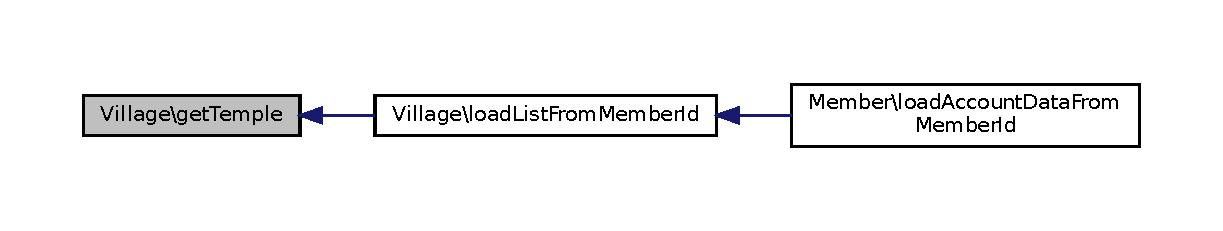
\includegraphics[width=350pt]{classVillage_a75b6534f378f19bb04147fd5c85a1de9_icgraph}
\end{center}
\end{figure}
\mbox{\Hypertarget{classVillage_a32709e6efc8c58dcedea9727cfa44973}\label{classVillage_a32709e6efc8c58dcedea9727cfa44973}} 
\index{Village@{Village}!load\+From\+Id@{load\+From\+Id}}
\index{load\+From\+Id@{load\+From\+Id}!Village@{Village}}
\subsubsection{\texorpdfstring{load\+From\+Id()}{loadFromId()}}
{\footnotesize\ttfamily Village\+::load\+From\+Id (\begin{DoxyParamCaption}{ }\end{DoxyParamCaption})}



This method load the data about this \mbox{\hyperlink{classVillage}{Village}} \+: 


\begin{DoxyItemize}
\item Workers in the \mbox{\hyperlink{classVillage}{Village}}
\item \mbox{\hyperlink{classTemple}{Temple}} in the \mbox{\hyperlink{classVillage}{Village}}
\item Buildings in the \mbox{\hyperlink{classVillage}{Village}} \begin{DoxyReturn}{Returns}
returns true if it\textquotesingle{}s succeed, false in the other case 
\end{DoxyReturn}

\end{DoxyItemize}Here is the caller graph for this function\+:
\nopagebreak
\begin{figure}[H]
\begin{center}
\leavevmode
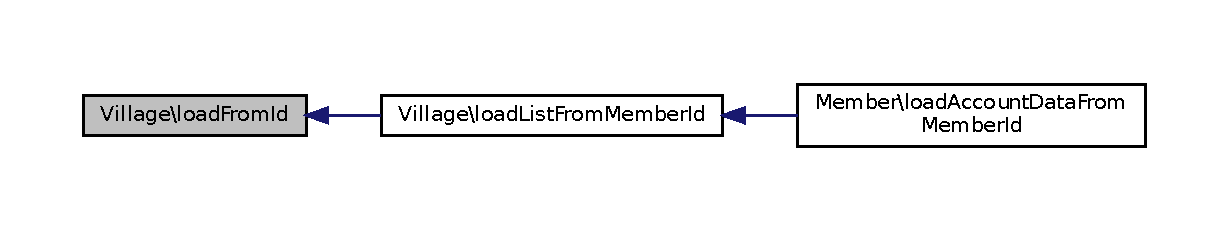
\includegraphics[width=350pt]{classVillage_a32709e6efc8c58dcedea9727cfa44973_icgraph}
\end{center}
\end{figure}
\mbox{\Hypertarget{classVillage_a1cedfa6d0cc4f8c432265c5b8309f931}\label{classVillage_a1cedfa6d0cc4f8c432265c5b8309f931}} 
\index{Village@{Village}!load\+List\+From\+Member\+Id@{load\+List\+From\+Member\+Id}}
\index{load\+List\+From\+Member\+Id@{load\+List\+From\+Member\+Id}!Village@{Village}}
\subsubsection{\texorpdfstring{load\+List\+From\+Member\+Id()}{loadListFromMemberId()}}
{\footnotesize\ttfamily static Village\+::load\+List\+From\+Member\+Id (\begin{DoxyParamCaption}\item[{}]{\$id }\end{DoxyParamCaption})\hspace{0.3cm}{\ttfamily [static]}}



This method load the data about all the \mbox{\hyperlink{classMember}{Member}} \mbox{\hyperlink{classVillage}{Village}} \+: 


\begin{DoxyItemize}
\item Workers in the \mbox{\hyperlink{classVillage}{Village}}
\item \mbox{\hyperlink{classTemple}{Temple}} in the \mbox{\hyperlink{classVillage}{Village}}
\item Buildings in the \mbox{\hyperlink{classVillage}{Village}} 
\begin{DoxyParams}{Parameters}
{\em id} & the \mbox{\hyperlink{classMember}{Member}} ID \\
\hline
\end{DoxyParams}
\begin{DoxyReturn}{Returns}
returns a list of \mbox{\hyperlink{classVillage}{Village}} if it\textquotesingle{}s succeed, false in the other case 
\end{DoxyReturn}

\end{DoxyItemize}Here is the call graph for this function\+:
\nopagebreak
\begin{figure}[H]
\begin{center}
\leavevmode
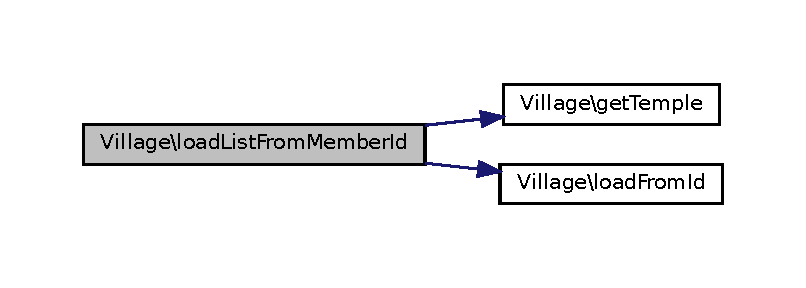
\includegraphics[width=350pt]{classVillage_a1cedfa6d0cc4f8c432265c5b8309f931_cgraph}
\end{center}
\end{figure}
Here is the caller graph for this function\+:
\nopagebreak
\begin{figure}[H]
\begin{center}
\leavevmode
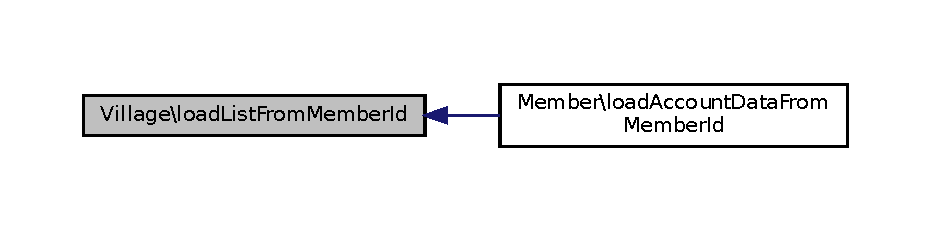
\includegraphics[width=350pt]{classVillage_a1cedfa6d0cc4f8c432265c5b8309f931_icgraph}
\end{center}
\end{figure}


The documentation for this class was generated from the following file\+:\begin{DoxyCompactItemize}
\item 
Classes/Village.\+php\end{DoxyCompactItemize}

\chapter{File Documentation}
\hypertarget{Controleurs_2accueil_8php}{}\section{Controleurs/accueil.php File Reference}
\label{Controleurs_2accueil_8php}\index{Controleurs/accueil.\+php@{Controleurs/accueil.\+php}}


This script manage two case \+:  


\subsection*{Variables}
\begin{DoxyCompactItemize}
\item 
\mbox{\Hypertarget{Controleurs_2accueil_8php_a60af369bff01e56fc0bf0677a6dff6cb}\label{Controleurs_2accueil_8php_a60af369bff01e56fc0bf0677a6dff6cb}} 
{\bfseries \$\+\_\+\+C\+SS} \mbox{[}$\,$\mbox{]} = \textquotesingle{}common.\+css\textquotesingle{}
\item 
\mbox{\Hypertarget{Controleurs_2accueil_8php_a43e5b5a819fedbd12b8cf5421ba6985e}\label{Controleurs_2accueil_8php_a43e5b5a819fedbd12b8cf5421ba6985e}} 
{\bfseries \$titre} = \textquotesingle{}Accueil\textquotesingle{}
\item 
\mbox{\Hypertarget{Controleurs_2accueil_8php_a1f34850a79fa25c790cf4189ff494b62}\label{Controleurs_2accueil_8php_a1f34850a79fa25c790cf4189ff494b62}} 
{\bfseries \$compte\+\_\+erreur} = false
\item 
\mbox{\Hypertarget{Controleurs_2accueil_8php_a90495ba52b30420e55824e8e1881b74a}\label{Controleurs_2accueil_8php_a90495ba52b30420e55824e8e1881b74a}} 
{\bfseries \$ressources} = array()
\item 
\mbox{\Hypertarget{Controleurs_2accueil_8php_a07a6a7957392eb99bec9d29e0ccc40e0}\label{Controleurs_2accueil_8php_a07a6a7957392eb99bec9d29e0ccc40e0}} 
{\bfseries \$village\+\_\+temple}
\item 
\mbox{\Hypertarget{Controleurs_2accueil_8php_a48d38ace588939a7197483e7911bc336}\label{Controleurs_2accueil_8php_a48d38ace588939a7197483e7911bc336}} 
if(isset(\$\+\_\+\+S\+E\+S\+S\+I\+ON\mbox{[}\textquotesingle{}id\textquotesingle{}\mbox{]})) {\bfseries \$donnees} = ob\+\_\+start()
\end{DoxyCompactItemize}


\subsection{Detailed Description}
This script manage two case \+: 


\begin{DoxyEnumerate}
\item A new visitor is coming, we have to show the connexion form
\item A member is now connected, we have to show his account resume 
\end{DoxyEnumerate}
\hypertarget{connexion_8php}{}\section{Controleurs/connexion.php File Reference}
\label{connexion_8php}\index{Controleurs/connexion.\+php@{Controleurs/connexion.\+php}}


This script job is te find if the member exist and store all data about it in S\+E\+S\+S\+I\+ON to limit the amount of needed \mbox{\hyperlink{classSQL}{S\+QL}} request on each page (0 until the member ask for some modifications)  




\subsection{Detailed Description}
This script job is te find if the member exist and store all data about it in S\+E\+S\+S\+I\+ON to limit the amount of needed \mbox{\hyperlink{classSQL}{S\+QL}} request on each page (0 until the member ask for some modifications) 


%--- End generated contents ---

% Index
\backmatter
\newpage
\phantomsection
\clearemptydoublepage
\addcontentsline{toc}{chapter}{Index}
\printindex

\end{document}
